\documentclass[11pt]{article}
\usepackage{amsmath,amssymb,amsthm}
\usepackage{bm}  % \mathbf does not bold Greek letters; \bm does
\usepackage{algorithm}
\usepackage{algpseudocode}
\usepackage{booktabs}
\usepackage{hyperref}
\usepackage{tikz}
\usepackage[style=numeric, sorting=none, backend=biber, url=false, doi=false, isbn=false, date=year]{biblatex}
\addbibresource{morl.bib}
% clean up the Zotero export here, so that re-exporting morl.bib does not undo it
\DeclareSourcemap{
  \maps[datatype=bibtex]{
    \map[overwrite=false]{  % keep the venue of entries that only have it as eventtitle
      \step[fieldsource=eventtitle, final]
      \step[fieldset=booktitle, origfieldval]
    }
    \map{  % repeated or unneeded venue details
      \step[fieldset=eventtitle, null]
      \step[fieldset=location, null]
      \step[fieldset=series, null]
    }
    \map{  % arXiv preprints: keep only the identifier, printed as "arXiv: 2206.11326"
      \step[fieldsource=eprinttype, match=arxiv, final]
      \step[fieldset=number, null]
      \step[fieldset=publisher, null]
    }
    \map{  % drop the category suffix, e.g. "2206.11326 [cs]"
      \step[fieldsource=eprint, match=\regexp{\s*\[.*\]}, replace={}]
    }
    \map[overwrite=true]{  % the Zotero entry has the title in capitals and no venue
      \step[fieldsource=entrykey, match=\regexp{^alver_constructing_2022$}, final]
      \step[typesource=article, typetarget=inproceedings]
      \step[fieldset=title, fieldvalue={Constructing a Good Behavior Basis for Transfer using Generalized Policy Updates}]
      \step[fieldset=booktitle, fieldvalue={International Conference on Learning Representations}]
    }
  }
}
\AtBeginBibliography{\sloppy}  % avoid the few lines that stick into the margin
\usetikzlibrary{arrows.meta}
\usepackage{graphicx}
\graphicspath{{figures/}}

\DeclareMathOperator{\argmax}{arg\,max}

% vector quantities
\newcommand{\vphi}{\bm{\phi}}      % vector reward
\newcommand{\vpsi}{\bm{\psi}}      % successor features
\newcommand{\vPsi}{\bm{\Psi}}
\newcommand{\vomega}{\bm{\omega}}  % state-dependent weight

\newtheorem{theorem}{Theorem}
\newtheorem{lemma}{Lemma}
\newtheorem{proposition}{Proposition}
\newtheorem{definition}{Definition}
\newtheorem{remark}{Remark}
\newtheorem{conjecture}{Conjecture}

\title{Faster convex coverage sets via metapolicies over base policies}
\author{Guillem Masdemont, Vicenç Gómez}
\date{\today}

\begin{document}
\maketitle


\begin{abstract}
    In Multi-Objective Reinforcement Learning, the Convex Coverage Set (CCS) combined with Generalized Policy Improvement (GPI) enables optimal transfer from a set of learnt tasks to unseen ones. However, reaching optimality often requires computing a large number of policies. This becomes infeasible in large MDPs, as the size of the CCS grows exponentially with the number of objectives. In this work, we present a metapolicy that chooses which base policy's action to take at every state, so that new policies can be composed from a small basis. The metapolicy is the optimal policy of the MDP restricted to the actions of the base policies, and its successor features are learned with a restricted form of SF Q-learning. This restriction trades the expressiveness of other approaches, such as the Option Keyboard, for efficient learning. We prove the convergence of our method and show that it reduces the number of samples needed to construct the CCS with respect to SFOLS, in both stochastic and deterministic domains. Furthermore, we propose a way to combine the metapolicy with GPI into a hybrid policy whose action values are provably at least those of GPI over the same basis, enabling better performance on unseen tasks when computing the whole CCS is still infeasible. These findings open new directions for optimal policy transfer in large domains, where only a small set of base policies can be computed in a reasonable amount of time.
\end{abstract}

\section{Introduction}

Multi-objective reinforcement learning (MORL) models Markov decision processes whose reward function signals several, often conflicting, objectives \cite{roijers_survey_2013,hayes_practical_2022}. The agent must act optimally under any possible preference weighting, hence, the relevant solution is the whole Pareto frontier of optimal value vectors, which is expensive to compute because it grows exponentially with the number of objectives. This motivates the \textit{optimal policy transfer} problem: achieving optimality on new tasks by combining previously learnt policies~\cite{alegre_optimistic_2022}.

In the linear case where the reward is a scalar product of objectives and weights, one can efficiently compute the value function of a policy across different tasks using successor features (SFs) \cite{roijers_multi-objective_2016, barreto_fast_2020}. Moreover, the optimal Pareto frontier forms a convex hull that can be leveraged using linear programming methods. While the learnt policies can be reused to improve performance on a new task, optimality depends on how diverse the basis set is. Zahavy et al.~\cite{zahavy_discovering_2021} construct this set iteratively by adding the policy that most improves the worst-case performance of the composed, set-max policy over all tasks. Alternatively, for deterministic dynamics and independent reward features, Alver and Precup~\cite{alver_constructing_2022} show that a set of independent policies, each maximizing its own feature without affecting the others, allows to maximize the expected return on every linearly task. Nevertheless, global optimallity is only guaranteed when the base policies forms a \textit{convex coverage set} (CCS), a minimal set of policies that contains an optimal policy for every preference \cite{roijers_multi-objective_2016}. Optimistic linear support (OLS) builds the CCS incrementally by solving the task at the corner weights of the current set \cite{roijers_multi-objective_2016}, and SFOLS \cite{alegre_optimistic_2022} combines it with SFs and \textit{General policy improvement} (GPI) to achieve optimality on every linear task. 

However, the number of policies that must be learned from scratch grows rapidly with the number of objectives, which makes SFOLS unfeasible in many domains. Recent works trade this guarantee for scalability: constructing a smaller behavior basis that is combined by a learned meta-policy, the option keyboard \cite{alegre_constructing_2025}, relying on independent policies \cite{alver_constructing_2022}, or discovering the features and approximating the SFs \cite{carvalho_combining_2023}. When the whole Pareto frontier is not even desirable one can restrict it with Lorenz dominance to favour specific reward distributions~\cite{michailidis_scalable_2026}.

In this work we reduce the cost of building the CCS by reusing previously learnt policies. Instead of learning a new policy from scratch, we try to compose it from a basis of previous policies through a \emph{metapolicy} that, at every state, chooses which base policy's action to take, and refines this choice by policy iteration. A Bellman certificate then checks whether the composed policy is already optimal for the queried weight. If it is not, then we learn the new policy and add it to the basis. In particular, this work demonstrates that:
\begin{itemize}
    \item Our \textsc{Certify-or-Grow} method recovers the same CCS as SFOLS with $3.2\times$ fewer environment steps until convergence than the warm-started SFOLS in the Deep Sea Treasure domain and $2.1\times$ fewer in the Office domain, averaged over 10 seeds, also when the certificate is checked without a model.
    \item The metapolicy can be extended with GPI and is provably at least as good as the GPI estimate over the same basis. In particular, we show in the stochastic double-slit domain it can be leveraged to greatly improve performance on a new task as a replacement of increasing the CCS.
\end{itemize}

We present results on both deterministic and stochastic environments, covering both Markovian and non-Markovian tasks. The Deep Sea Treasure domain is taken from the MORL benchmarking toolkit \cite{felten_toolkit_2023}, while the Office and double slit domains come from Kuric et al. \cite{kuric_planning_2024}. In the non-Markovian setting, learned SFs are composed over a finite state automaton \cite{kuric_planning_2024}, in the spirit of options \cite{sutton_between_1999} and reward machines \cite{li_reward_2024}. The remainder of the work is structured as follows. In Sec.~\ref{sec:Background} we introduce the notation, SFs, GPI and the CCS. In Sec.~\ref{sec:Formalism} we define the metapolicy, the Bellman certificate and \textsc{Certify-or-Grow}, and show that the hybrid policy improves on GPI. In Sec.~\ref{sec:results} we evaluate our method in the Deep Sea Treasure, Office and double slit domains. We conclude in Sec.~\ref{sec:conclusions}.

\section{Background and notation}\label{sec:Background}


An MDP is a tuple $\mathcal{M} = (S, A, P, r, \gamma)$, where $S$ is the state space, $A$ is the action space, $P(\cdot | s, a)$ is the transition distribution from taking action $a$ at state $s$, $r : S \times A \times S \to \mathbb{R}$ is the reward function, and $\gamma \in [0,1)$ is the discount factor. In the context of MORL, we consider a vector reward function with $d$ objectives represented by a feature vector $\vphi(s,a,s') \in \mathbb{R}^d$. Every MORL problem induces a family of MDPs via a scalarization function that maps the vector of objectives to a scalar reward \cite{roijers_survey_2013}. In the linear case, every weight $\mathbf{w}$ induces a task, given by the MDP $\mathcal{M}_{\mathbf{w}} = (S, A, P, r_{\mathbf{w}}, \gamma)$ with reward $r_{\mathbf{w}}(s, a, s') = \vphi(s, a, s') \cdot \mathbf{w}.$ We denote by $V^*_{\mathbf{w}}$ the optimal value function of $\mathcal{M}_{\mathbf{w}}$, and by $\pi^*_{\mathbf{w}}$ an optimal policy.

Without loss of generality, we can assume that $\mathbf{w}$ is a probability distribution, i.e., $\mathbf{w} \in \Delta(d)$, where $\Delta(d) = \{\mathbf{w} \in \mathbb{R}^d \,|\, \sum_{i=1}^d w_i = 1, w_i \geq 0 \}$. Negative weights are also considered in other works \cite{barreto_fast_2020}, however, in that case the optimal policies are no longer restricted to the Pareto frontier, and the methods that rely on its convexity do not apply directly \cite{moffaert_multi-objective_2014,michailidis_scalable_2026}. In this work the features $\vphi$ are given, although in more general settings they can also be learned from experience together with weights \cite{barreto_fast_2020,carvalho_combining_2023}.

Given a policy $\pi$, we define its successor features (SFs) \cite{barreto_successor_2017} by
\begin{equation}
    \vpsi^\pi(s,a) = \mathbb{E}_\pi \left[ \sum_{t = 0}^\infty \gamma^t \vphi(s_t, a_t, s_{t+1}) \,\Big|\, s_0 = s, a_0 = a \right].
\end{equation}
The linearity in the reward allows $q_{\mathbf{w}}^\pi(s,a) = \vpsi^\pi(s,a) \cdot \mathbf{w}$. Moreover, the SFs satisfy the Bellman equation $\vpsi^\pi(s,a) = \mathbb{E}_{s'}\left[\vphi(s,a,s') + \gamma \vpsi^\pi(s', \pi(s'))\right]$, so they can be computed with policy evaluation or learned with temporal-difference methods.

Given a set of policies $\Pi = \{\pi_i\}_{i = 1}^N$ and their corresponding successor features $\{\vpsi^{\pi_i}(s,a)\}$, generalized policy improvement (GPI) \cite{barreto_successor_2017} defines a new policy via
\begin{equation}\label{eq:gpi}
    \pi^{GPI}(s) = \arg \max_{a \in A} \max_{\pi \in \Pi} \vpsi^{\pi}(s,a) \cdot \mathbf{w}.
\end{equation}
For any weight $\mathbf{w}$, $\pi^{GPI}$ is proven to perform at least as well as all the policies in $\Pi$, because $q_{\mathbf{w}}^{\pi^{GPI}}(s,a) \geq \max_{\pi \in \Pi} q_{\mathbf{w}}^{\pi}(s,a)$ for every $(s,a) \in S \times A$. Note that GPI is a one-step improvement: it evaluates every action assuming that a single policy of $\Pi$ is followed afterwards. In general it is not optimal and it can perform poorly when the optimal behaviour requires switching between policies \cite{hunt_composing_2019}. However, GPI is guaranteed to be optimal if $\Pi$ covers all the possible optimal behaviours, i.e., if for any weight $\mathbf{w}$ there exists $\pi \in \Pi$ optimal for $\mathcal{M}_{\mathbf{w}}$. Given an initial state distribution $\nu_0$, let $\vpsi^\pi = \mathbb{E}_{s \sim \nu_0} \left[ \vpsi^\pi(s, \pi(s)) \right]$ be the expected return vector of $\pi$. The optimal policies from $\nu_0$ lie in the Pareto frontier given by the dominance relation $\vpsi^\pi \preceq \vpsi^{\pi'} \iff \psi^\pi_i \leq \psi^{\pi'}_i$ for all $i \in \{1, \dots, d\}$. For the linear case it is enough to keep its convex part, the \textit{convex coverage set} (CCS) \cite{roijers_multi-objective_2016,alegre_optimistic_2022}, which contains the return vectors that are optimal for some task:
\begin{equation}
    CCS = \left \{\vpsi^\pi \,\middle|\, \exists \mathbf{w} \in \Delta(d) \ \text{such that} \ \vpsi^\pi \cdot \mathbf{w} \geq \vpsi^{\pi'} \cdot \mathbf{w} \ \ \forall \pi' \right \}.
\end{equation}
If $\Pi$ contains the policies that define the CCS, then $\pi^{GPI}$ is optimal for every weight \cite{alegre_optimistic_2022}. Note that the CCS is defined with respect to $\nu_0$, so it is important to have a good distribution of initial states if one wants optimality from every initial condition, otherwise the CCS may miss optimal policies for unexplored initial states.

Given a partial CCS, $\max_{\pi \in \Pi} \vpsi^\pi \cdot \mathbf{w}$ is a piecewise-linear convex function of $\mathbf{w}$, and its \textit{corner weights} are the weights where the linear pieces intersect, namely, the vertices of the polytope $\{(\mathbf{w}, v) \,|\, \mathbf{w} \in \Delta(d),\ v \geq \vpsi^\pi \cdot \mathbf{w}\ \forall \pi \in \Pi\}$. 

\begin{theorem}[\cite{roijers_multi-objective_2016}]\label{thm:corner}
    Given a set of policies $\Pi$, the maximum gap between the optimal value and the value of $\Pi$,
    \begin{equation}
        \max_{\mathbf{w} \in \Delta(d)} \left( V^*_{\mathbf{w}} - \max_{\pi \in \Pi} \vpsi^\pi \cdot \mathbf{w} \right),
    \end{equation}
    is always attained at a corner weight of $\Pi$.
\end{theorem}

Theorem \ref{thm:corner} ensures that if the optimal policy of every corner weight is already in $\Pi$, the set is a CCS. Optimistic linear support (OLS) \cite{roijers_multi-objective_2016} uses this to build the CCS incrementally by starting in the extreme weights and querying corner weights until no improvement. SFOLS (Algorithm~\ref{alg:sfols}) combines OLS with SFs and GPI \cite{alegre_optimistic_2022}. Each queried weight is solved starting from the GPI policy over the policies learned so far, and the corner weights are prioritized by an upper bound on their gap, so that the most informative one is explored first. The order of the queries does not affect convergence, but it can improve its speed, since a weight close to an already explored one may give the same optimal policy, and hence the same SFs. Other prioritizations are proposed in \cite{alegre_sample-efficient_2023}.

\begin{algorithm}[H]
\caption{SFOLS \cite{alegre_optimistic_2022}}\label{alg:sfols}
\begin{algorithmic}[1]
\State $\Pi \gets \emptyset$, $CCS \gets \emptyset$, $Q \gets \{\mathbf{e}_1, \dots, \mathbf{e}_d\}$ \Comment{queue of weights to query}
\While{$Q \neq \emptyset$}
    \State $\mathbf{w} \gets$ pop weight of $Q$ with highest priority
    \State $\pi_{\mathbf{w}}, \vpsi^{\pi_{\mathbf{w}}} \gets$ solve $\mathcal{M}_{\mathbf{w}}$ \label{alg:sfols-solve}
    \State $\Pi \gets \Pi \cup \{\pi_{\mathbf{w}}\}$
    \If{$\vpsi^{\pi_{\mathbf{w}}} \notin CCS$ and it improves $\max_{\pi \in \Pi}\vpsi^\pi \cdot \mathbf{w}$}
        \State $CCS \gets CCS \cup \{\vpsi^{\pi_{\mathbf{w}}}\}$, and remove the corner weights of $Q$ that are no longer corners
        \State add the new corner weights to $Q$, with priority given by an upper bound on their gap
    \EndIf
\EndWhile
\State \Return $CCS$, $\Pi$
\end{algorithmic}
\end{algorithm}

SFOLS often performs redundant solves. For example, the Deep Sea Treasure environment \cite{cassimon_review_2024} needs 19 weight solves, of which only 10 yield different policies. Moreover, the size of the CCS grows exponentially with the number of objectives, so in many cases computing it is very expensive and not even necessary. For example, in the Office domain \cite{kuric_planning_2024}, the policies of the $d$ extreme weights are already enough to achieve zero-shot optimality with GPI. The reason is that, in most problems, the optimal policy for a new weight is the behaviour of a few base policies over broad regions of the state space, and only switches between them at specific states. Hence, a new policy often does not need to be learned from scratch, as long as we can decide when the cached policies are enough. Nemecek and Parr \cite{nemecek_policy_2021} address this decision with bounds on the optimal value of a new task, which tell whether to reuse the cached policies with GPI or to learn a new one.


Recent works reduce the number of policies in the basis, in exchange for a richer way of combining them. Some works build the basis from the eigenvectors of the graph Laplacian of the environment and combine it with GPI \cite{chandrasekar_towards_2025}, while others learn a successor feature approximator jointly with the features and the weights \cite{borsa_universal_2018,carvalho_combining_2023}. The Option Keyboard \cite{barreto_option_2021} combines a basis of options through a learned metapolicy that outputs, at each state, the weight used to compose them with GPI, and Alegre et al. \cite{alegre_constructing_2025} recently showed how to construct a basis for it that is optimal for every task.
\begin{equation}\label{eq:option_keyboard}
    \pi^{OK}(s) = \arg \max_{a \in A} \max_{\pi \in \Pi} \vpsi^{\pi}(s,a) \cdot \vomega(s, \mathbf{w}),
\end{equation}
where $\vomega: S \times \Delta(d) \to \mathbb{R}^d$ is a trained metapolicy. Changing the weight at each state allows $\pi^{OK}$ to produce behaviours that no base policy has. However, learning $\vomega$ is usually hard since the optimal policy is mostly a composition of base policies over broad regions and the target $\vomega$ becomes a step function. Moreover, the $\arg\max$ in Eq.~\eqref{eq:option_keyboard} partitions the weight space into a mesh of open cells, each of them selecting an action. Hence, small enough changes on $\vomega$ do not change the action output and the gradient vanishes. Finally, Eq.~\eqref{eq:option_keyboard} does not restrict the actions to those of the base policies, so for $\omega$ to reach the cell of the optimal action, the learning process may have to move through cells whose actions are not optimal.

In this paper, we exploit these observations and present a metapolicy for MDPs that only allows, at each state, the actions of the base policies. Since each base policy $\pi_j$ is optimal for its training weight $\mathbf{w}_j$, taking $\vomega(s, \mathbf{w}) = \mathbf{w}_j$ in Eq.~\eqref{eq:option_keyboard} recovers exactly the action $\pi_j(s)$, so this is equivalent to restricting the option keyboard to discrete choices. This discrete choice can be learned efficiently, and it proves to be faster than SFOLS in the Deep Sea Treasure and Office domains. %Moreover, it comes with a certificate of optimality that tells when a new policy must be learned.ƒ


\section{Formalism}\label{sec:Formalism}

We first describe how to compute a metapolicy from a set of base policies, then detail the construction of the CCS. Throughout this section, the query weight $\mathbf{w}$ remains fixed.

\subsection{Metapolicy}

We call \textit{basis} a finite set of policies $\mathcal{B} = \{\pi_j\}_{j=1}^k$, together with their successor features $\{\vpsi^{\pi_j}(s,a)\}$. Each $\pi_j$ is optimal for its own training weight $\mathbf{w}_j$, hence, $\pi_j(s) = \arg\max_{a \in A} \vpsi^{\pi_j}(s,a) \cdot \mathbf{w}_j$. 

For any state $s$, consider the restricted action set given by the actions of the base policies:
\begin{equation}
    B(s) = \{\pi_1(s), \dots, \pi_k(s)\} \subseteq A.
\end{equation}
and define $\mathcal{M}_{\mathcal{B}}$ as the MDP with the same states, transitions and features as $\mathcal{M}$, but with action set $B(s)$ at every state. In $\mathcal{M}_{\mathcal{B}}$ the agent chooses which base policy to follow at each state. Since the optimal policy is often a composition of the base policies over broad regions, it is frequently contained in $\mathcal{M}_{\mathcal{B}}$.

We define the \textit{metapolicy} $\pi_{\mathrm{meta}}$ over $\mathcal{B}$ as the optimal policy of $\mathcal{M}_{\mathcal{B}}$ for the weight $\mathbf{w}$, and $V_{\mathrm{meta}}$ as its value. For any value function $V$, we write the one-step backup as
\begin{equation}
    Q_V(s,a) = \mathbb{E}_{s' \sim P(\cdot|s,a)} \left[ \vphi(s,a,s') \cdot \mathbf{w} + \gamma V(s') \right],
\end{equation}
The Bellman optimality operator of $\mathcal{M}_{\mathbf{w}}$ is $(TV)(s) = \max_{a \in A} Q_V(s,a)$, with unique fixed point $V^*_{\mathbf{w}}$. Equivalently, $V_{\mathrm{meta}}$ is the unique fixed point of the restricted Bellman operator
\begin{equation}
    (T_B V)(s) : = \max_{a \in B(s)} Q_V(s,a) = \max_{j \in \{1,\dots,k\}} Q_V(s, \pi_j(s)),
\end{equation}
which is also a $\gamma$-contraction, and the metapolicy follows, at each state, the best base policy:
\begin{equation}\label{eq:metapolicy}
    \pi_{\mathrm{meta}}(s) = \pi_{j^*(s)}(s), \qquad j^*(s) = \arg\max_{j \in \{1,\dots,k\}} Q_{V_{\mathrm{meta}}}(s, \pi_j(s)).
\end{equation}
Note that the metapolicy can never pick an action that none of the base policies would take. Moreover, since every base policy is itself a policy of $\mathcal{M}_{\mathcal{B}}$, the metapolicy is at least as good as all of them.

\begin{lemma}[$V_{\mathrm{meta}}$ dominates the base policies]\label{lem:meta-dominates}
    For every base policy $\pi_j \in \mathcal{B}$ and every state $s$, $V_{\mathrm{meta}}(s) \geq V^{\pi_j}(s)$, where $V^{\pi_j}(s) = \vpsi^{\pi_j}(s, \pi_j(s)) \cdot \mathbf{w}$.
\end{lemma}
\begin{proof}
    Since $\pi_j(s) \in B(s)$, the Bellman equation of $\pi_j$ gives $V^{\pi_j}(s) = Q_{V^{\pi_j}}(s, \pi_j(s)) \leq (T_B V^{\pi_j})(s)$. Applying the monotone operator $T_B$ repeatedly gives a non-decreasing sequence $V^{\pi_j} \leq T_B V^{\pi_j} \leq T_B^2 V^{\pi_j} \leq \dots$, which converges to $V_{\mathrm{meta}}$ by the contraction property.
\end{proof}

\subsection{Learning the metapolicy and its successor features}

In practice, we focus on learning the SFs of $\pi^{meta}$ rather than its value function as SFs are required to perform GPI. Hence, instead of iterating $T_B$ and then evaluating the resulting policy, we learn both at once with SF Q-learning \cite{barreto_fast_2020}, where the bootstrap is restricted to the actions of the base policies (Algorithm~\ref{alg:metapolicy-ql}).

\begin{algorithm}[H]
\caption{\textsc{MetaPolicy}$(\mathcal{B},\mathbf{w})$}\label{alg:metapolicy-ql}
\begin{algorithmic}[1]
\State $\widehat\vpsi(s,a) \gets \vpsi^{\pi_{j}}(s,a)$ with $j = \arg\max_j \vpsi^{\pi_j}(s,a) \cdot \mathbf{w}$, for every $(s,a)$
\Repeat
  \State observe $(s,a,\vphi(s,a,s'),s')$ under a behaviour policy with enough state-action coverage
  \State $\hat\jmath \gets \arg\max_{j\in\{1,\dots,k\}} \widehat\vpsi\big(s',\pi_j(s')\big) \cdot \mathbf{w}$
  \State $\widehat\vpsi(s,a) \gets \widehat\vpsi(s,a) + \alpha\,\big[\vphi(s,a,s') + \gamma\,\widehat\vpsi\big(s',\pi_{\hat\jmath}(s')\big)-\widehat\vpsi(s,a)\big]$
\Until{converged}
\State $\pi_{\mathrm{meta}}(s) \gets \pi_{j^*(s)}(s)$, with $j^*(s) = \arg\max_j\widehat\vpsi(s,\pi_j(s)) \cdot \mathbf{w}$, for every $s$
\State \Return $\pi_{\mathrm{meta}}$, $\widehat\vpsi$
\end{algorithmic}
\end{algorithm}

The update has two parts: The $\arg\max$ of the target only ranges over $B(s')$, therefore, the scalar values $\widehat\vpsi(s,a) \cdot \mathbf{w}$ follow exactly the Q-learning update of $\mathcal{M}_{\mathcal{B}}$. Hence they converge to $V_{\mathrm{meta}}$, and the greedy choice $\hat\jmath$ converges to the metapolicy of Eq.~\eqref{eq:metapolicy}. Second, the scalar values also converge for every pair $(s,a)$ visited by the behaviour policy, including the actions $a \notin B(s)$, and if the best action of $\mathcal{M}_{\mathcal{B}}$ is unique at every state, $\widehat\vpsi$ converges to $\vpsi^{\pi_{\mathrm{meta}}}(s,a)$. We prove both results, and discuss the case of ties, in Appendix~\ref{app:convergence}. Algorithm \ref{alg:metapolicy-ql} can be speeded-up by improving sample efficiency, as described in \cite{alegre_sample-efficient_2023}. The table can also be warm started with GPI over the basis together with all the metapolicies certified so far.

\subsection{Bellman certificate}

The metapolicy is optimal on $\mathcal{M}_{\mathcal{B}}$, but not necessarily on $\mathcal{M}$, since the optimal policy may need an action that is not in $B(s)$. We define the optimality gap as $\mathrm{gap}_{\mathbf{w}}(s) = (T V_{\mathrm{meta}})(s) - V_{\mathrm{meta}}(s)$. Here $T$ is the unrestricted Bellman operator. This gap can be read directly from the table returned by Algorithm~\ref{alg:metapolicy-ql} as 
\begin{equation}\label{eq:gap}
    \mathrm{gap}_{\mathbf{w}}(s) = \max_{a \in A} \vpsi^{\pi_{\mathrm{meta}}}(s,a) \cdot \mathbf{w} - \vpsi^{\pi_{\mathrm{meta}}}(s, \pi_{\mathrm{meta}}(s)) \cdot \mathbf{w}.
\end{equation}
Note that $\mathrm{gap}_{\mathbf{w}}(s) \geq 0$ for every state, because $B(s) \subseteq A$. If the gap is zero at every state, then $V_{\mathrm{meta}}$ is also a fixed point of $T$, hence $V_{\mathrm{meta}} = V^*_{\mathbf{w}}$ and the metapolicy is optimal for $\mathbf{w}$. More generally, if $\max_s \mathrm{gap}_{\mathbf{w}}(s) \leq \varepsilon$, the contraction of $T$ gives
\begin{equation}\label{eq:certificate}
\begin{aligned}
    \| V^*_{\mathbf{w}} - V_{\mathrm{meta}} \|_\infty &\leq \| T V^*_{\mathbf{w}} - T V_{\mathrm{meta}} \|_\infty + \| T V_{\mathrm{meta}} - V_{\mathrm{meta}} \|_\infty \\
    &\leq \gamma \| V^*_{\mathbf{w}} - V_{\mathrm{meta}} \|_\infty + \varepsilon,
\end{aligned}
\end{equation}
so the metapolicy is $\varepsilon / (1-\gamma)$-optimal. 

Note that Eq.~\eqref{eq:gap} needs $\vpsi^{\pi_{\mathrm{meta}}}(s,a)$ also for the actions outside $B(s)$, which Algorithm~\ref{alg:metapolicy-ql} does not visit. Once $\pi_{\mathrm{meta}}$ is learned, each of them follows from a single backup, $\vpsi^{\pi_{\mathrm{meta}}}(s,a) = \mathbb{E}_{s'}\left[\vphi(s,a,s') + \gamma \vpsi^{\pi_{\mathrm{meta}}}(s', \pi_{\mathrm{meta}}(s'))\right]$, since the right-hand side only uses entries of the actions in $B(s')$, which are already learned. With a known model this backup is computed directly. Without it, we take each missing action once and use the observed transition, which is exact in deterministic domains; in stochastic domains a few samples per pair have to be averaged. These extra samples are counted in our results.

\subsection{\textsc{Certify-or-Grow}}

We now present \textsc{Certify-or-Grow} (Algorithm~\ref{alg:certify-or-grow}), which uses the certificate to answer a query weight. It first learns the metapolicy over the current basis. If the certificate holds, the metapolicy is returned without learning any new policy. Otherwise, we solve the task at $\mathbf{w}$ over the full action set, and the new policy is added to the basis, so that the next queries can reuse it.

\begin{algorithm}[H]
\caption{\textsc{Certify-or-Grow}$(\mathbf{w},\mathcal{B})$}\label{alg:certify-or-grow}
\begin{algorithmic}[1]
\State $\pi_{\mathrm{meta}},\ \vpsi^{\pi_{\mathrm{meta}}} \gets \textsc{MetaPolicy}(\mathcal{B}, \mathbf{w})$ \Comment{Algorithm~\ref{alg:metapolicy-ql}}
\If{$\max_s \mathrm{gap}_{\mathbf{w}}(s) \le \varepsilon$} \Comment{Eq.~\eqref{eq:gap}}
    \State \Return $\pi_{\mathrm{meta}},\ \vpsi^{\pi_{\mathrm{meta}}},\ \mathcal{B}$
\Else
    \State $\pi_{\mathbf{w}},\ \vpsi^{\pi_{\mathbf{w}}} \gets$ solve $\mathcal{M}_{\mathbf{w}}$ over the full action set \label{alg:cog-fallback}
    \State $\mathcal{B}\gets\mathcal{B}\cup\{\pi_{\mathbf{w}}\}$
    \State \Return $\pi_{\mathbf{w}},\ \vpsi^{\pi_{\mathbf{w}}},\ \mathcal{B}$
\EndIf
\end{algorithmic}
\end{algorithm}

To build the CCS, the OLS loop of SFOLS (Algorithm~\ref{alg:sfols}) remains unchanged, and we only replace the solve at each corner weight (line~\ref{alg:sfols-solve}) by Algorithm~\ref{alg:certify-or-grow}. Since a certified metapolicy is optimal for its weight, the CCS obtained is the same as with SFOLS, but many of its elements are composed instead of learned from scratch.

\subsection{Combining the metapolicy with GPI}

The metapolicy might not beat GPI over the same basis because GPI can also pick actions that no base policy would ever take. We now define a policy that combines both. We call \textit{instant GPI value} the quantity that GPI maximizes, $Q^{GPI}_{\mathbf{w}}(s,a) = \max_j \vpsi^{\pi_j}(s,a) \cdot \mathbf{w}$, so that $\pi^{GPI}(s) = \arg\max_a Q^{GPI}_{\mathbf{w}}(s,a)$. For every $j$ and action $a \in A$, the immediate reward of $Q^{\pi_j}_{\mathbf{w}}(s,a)$ does not depend on $j$, hence
\begin{equation}\label{eq:gpi-decomposition}
    Q^{GPI}_{\mathbf{w}}(s,a) = \mathbb{E}_{s'}\left[ \vphi(s,a,s') \cdot \mathbf{w} \right] + \gamma \max_j \mathbb{E}_{s'}\left[ V^{\pi_j}(s') \right].
\end{equation}

That is, GPI evaluates every action by following a single base policy afterwards. By Lemma~\ref{lem:meta-dominates}, substituting $V^{\pi_j}$ by $V_{\mathrm{meta}}$ in Eq.~\eqref{eq:gpi-decomposition} can only increase it, and by the Bellman equation of $\pi_{\mathrm{meta}}$ the result is its action value. Hence
\begin{equation}\label{eq:gpi-bound}
    Q^{GPI}_{\mathbf{w}}(s,a) \leq Q^{\mathrm{meta}}_{\mathbf{w}}(s,a) = \vpsi^{\pi_{\mathrm{meta}}}(s,a) \cdot \mathbf{w} \quad \forall (s,a).
\end{equation}

This motivates the \textit{hybrid policy}, which can take any action of $A$ but scores it with the value of the metapolicy:
\begin{equation}\label{eq:hyb}
    \pi^{\mathrm{hyb}}(s) = \arg\max_{a \in A} \vpsi^{\pi_{\mathrm{meta}}}(s,a) \cdot \mathbf{w}.
\end{equation}

Since $\pi^{\mathrm{hyb}}$ is greedy with respect to $Q^{\mathrm{meta}}_{\mathbf{w}}$, the policy improvement theorem gives $Q^{\pi^{\mathrm{hyb}}}_{\mathbf{w}} \geq Q^{\mathrm{meta}}_{\mathbf{w}} \geq Q^{GPI}_{\mathbf{w}}$, namely, the hybrid policy always achieves at least the instant GPI value. However, this does not guarantee that $\pi^{\mathrm{hyb}}$ beats the policy $\pi^{GPI}$ when it is executed. Both policies score each action assuming a fixed continuation, the metapolicy or a single base policy, but when executed they choose again at every state over the full action set, and their actual continuation can be better than the one they assumed. Hence, $\pi^{GPI}$ can occasionally reach states where such an improvement is larger, and obtain more than $\pi^{\mathrm{hyb}}$. Nevertheless, this is rare in practice: over the tested weights, $\pi^{\mathrm{hyb}}$ never performed worse than $\pi^{GPI}$ in the Deep Sea Treasure and Office domains
Moreover, $\pi^{\mathrm{hyb}}$ is just the greedy policy of the table $\vpsi^{\pi_{\mathrm{meta}}}$ over the full action set, which \textsc{Certify-or-Grow} already computes, so it comes for free on top of our algorithm.

Hence, the hybrid policy can be used in two ways. When the certificate fails, it can help warm start the solve of line~\ref{alg:cog-fallback} in Algorithm~\ref{alg:certify-or-grow}, and in the same way that \cite{zahavy_discovering_2021} uses the value of the set-max policy $v^{\mathrm{SMP}}$, it can be used as a heuristic to choose which weights to explore. Moreover, when building the whole CCS is not feasible, $\pi^{\mathrm{hyb}}$ can be used directly on a new task as a replacement for growing the basis, as we show in the double slit domain in Sec.~\ref{sec:results}.

\section{SF-FSA-VI algorithm}\label{sec:fsa}

We now use the previous sections to build a complete algorithm for SF-FSA-VI \cite{kuric_planning_2024}. In this setting, the low-level MDP has $d$ exit states $\mathcal{E} = \{\varepsilon_1, \dots, \varepsilon_d\}$, and the feature vector is $\vphi(s,a,s') = \mathbf{e}_j$ when $s' = \varepsilon_j$ and $\mathbf{0}$ otherwise. The task is a finite state automaton with states $\mathcal{U}$, where reaching the exit $\varepsilon_j$ in state $u$ moves the automaton to $\tau(u,j)$. SF-FSA-VI computes a weight vector $\mathbf{w}(u)$ for every $u \in \mathcal{U}$ by iterating
\begin{equation}\label{eq:sf-fsa-vi}
    w^{k+1}_j(u) = \max_{a \in A} \max_{\pi \in \Pi} \vpsi^{\pi}(\varepsilon_j, a) \cdot \mathbf{w}^k\big(\tau(u,j)\big),
\end{equation}
with $w_j(u) = 1$ when $\tau(u,j)$ is the accepting state, and then acts with GPI at $\mathbf{w}(u)$ in every automaton state. Its main bottleneck is that Eq.~\eqref{eq:sf-fsa-vi} is only exact when $\Pi$ is a CCS. In this section we show that, when the low-level MDP is deterministic, the $d$ policies of the extreme weights $\mathbf{e}_1, \dots, \mathbf{e}_d$ are enough to achieve optimality for any weight. Under stochastic transitions they are not, and we leverage the metapolicy to improve the algorithm.

\subsection{SF-FSA-VI for deterministic domains}

\begin{theorem}\label{thm:det}
    Let the low-level MDP be deterministic, with the exit features above, and let $\pi_k$ be an optimal policy for $\mathbf{e}_k$, for $k = 1, \dots, d$. Then, for every $(s,a)$ and every weight $\mathbf{w} \in \Delta(d)$: 
    \begin{equation}
        \max_{k} \vpsi^{\pi_k}(s,a) \cdot \mathbf{w} = Q^{*}_{\mathbf{w}}(s,a).
    \end{equation}
    As a consequence, GPI over the $d$ extreme policies is optimal for every weight, and SF-FSA-VI over them is optimal for every task.
\end{theorem}

\begin{proof}
    Under the hypothesis, $Q^*_{\mathbf{w}}(s,a)$ ends in at most one exit, say $\varepsilon_k$ after $t$ steps, hemce, returns $w_k \gamma^t$. If the sequence never ends returns $0$ which is worse. Moreover, the best way to reach $\varepsilon_k$ is the fastest one, whose discounted value is $\psi^{\pi_k}_k(s,a)$. Hence $Q^*_{\mathbf{w}}(s,a) = \max_k w_k \psi^{\pi_k}_k(s,a)$. On the other hand, since the features and the weights are non-negative, $\vpsi^{\pi_k}(s,a) \cdot \mathbf{w} \geq w_k \psi^{\pi_k}_k(s,a)$, so $\max_k \vpsi^{\pi_k}(s,a) \cdot \mathbf{w} \geq Q^*_{\mathbf{w}}(s,a)$. Finally, $\vpsi^{\pi_k}(s,a) \cdot \mathbf{w} = Q^{\pi_k}_{\mathbf{w}}(s,a) \leq Q^*_{\mathbf{w}}(s,a)$, and the sandwich argument gives the equality. 
\end{proof}

Moreover, since $\pi_k(s)$ is the first step of a fastest path to $\varepsilon_k$, the optimal action at every state is the action of one of the extreme policies, so $B(s)$ contains it and the metapolicy over the $d$ extreme policies is also optimal. Hence, the algorithm of \cite{kuric_planning_2024} can be used unchanged with only the $d$ extreme policies, and each iteration costs $|\mathcal{U}||\mathcal{E}|d$ instead of $|\mathcal{U}||\mathcal{E}||\Pi_{CCS}|$. Note that this requires the extreme policies to be optimal from every exit, so their initial state distribution $\nu_0$ must cover the exits, as \cite{kuric_planning_2024} assume with $\mathcal{E} \subset \mathrm{supp}(\nu_0)$. 

This does not hold for stochastic transitions because a policy can then split its probability between exits, and its return becomes a weighted sum over them, $\sum_k w_k \mathbb{E}[\gamma^{T}\mathbf{1}\{\text{exit } k\}]$, with $T$ the exit time, which can exceed $\max_k w_k  \psi^{\pi_k}_k(s,a)$. For example, in the double slit domain (Figure~\ref{fig:double_slit}a), the optimum keeps several exits open. 

\subsection{SF-FSA-VI for stochastic domains}

In such environments, the extreme policies are not sufficient to complete every task optimally, since the optimal Q-function is no longer attained by a single exit. Hence, zero-shot optimality requires the whole CCS. On the other hand, GPI can achieve the optimal policy with far fewer policies than the whole CCS. However, the backward propagation of SF-FSA-VI makes us compute the whole CCS, because it needs not only the optimal policy for each weight, but also its value at the exits. Given this, we propose an algorithm....



\section{Results}\label{sec:results}

We present results on Algorithm~\ref{alg:certify-or-grow} for the Deep Sea Treasure and Office domains~\cite{cassimon_review_2024,felten_toolkit_2023, kuric_planning_2024}. As baselines, we take the standard SFOLS algorithm~\cite{alegre_optimistic_2022} and a warm-started version where the SF table of each new weight is initialized with GPI over all the policies learned so far. We compare them with two versions of \textsc{Certify-or-Grow}, both warm started. The first one checks the Bellman certificate with the model, while the second assumes a model-free version and completes the table outside $B(s)$ with sampling transitions. All methods learn the SFs with the same tabular SF Q-learning, with $\gamma = 0.99$, $\alpha = 1$ (domain is deterministic) and $\varepsilon = 0.1$, we stop the learning once every allowed state-action pair doesn't change under a certain tolerance in the SFs, as checking the Q-values is not enough since components with zero weight would never be checked. This stopping rule is conservative and chosen by simplicity, hence, we report both: the steps until the last change (suppossing that an oracle tells when the SFs converged) and all the environment steps used in the conservative rule. In the Office domain the full CCS is too large, so we compute an $\varepsilon$-CCS with $\varepsilon = 0.05$. Results are presented in Figure~\ref{fig:ccs_cost}.

\begin{figure}[htbp]
    \centering
    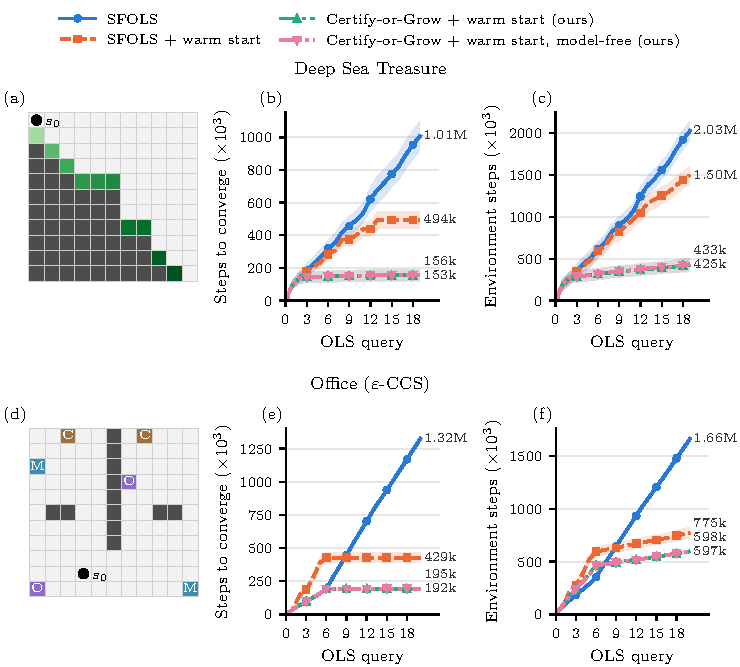
\includegraphics[width=\textwidth]{q_ccs_cost.pdf}
    \caption{Cumulative sample cost of building the CCS with learned successor features as a function of the OLS query, in the Deep Sea Treasure (top) and Office (bottom). All methods recover the same CCS as with exact successor features. (a) Deep Sea Treasure: the agent starts at $s_0$ and each treasure ends the episode. (d) Office: walls in dark grey and the six objects (two coffees C, two offices O and two mail M); episodes start at $s_0$ or at one of the objects. (b, e) Environment steps until convergence. (c, f) All environment steps, including confirming convergence. Mean over 10 seeds, shaded band is $\pm 1$ standard deviation. In Office the variance across seeds is very small, and only the first 20 of the 63 OLS queries of the $\varepsilon$-CCS are shown.}
    \label{fig:ccs_cost}
\end{figure}


All methods recover the same CCS with exact SFs on every seed. However, \textsc{Certify-or-Grow} needs far fewer samples. We compare the steps until convergence (Figure~\ref{fig:ccs_cost}b,e), since the total number of steps also depends on the stopping rule, which is not necessarily the same for every method. In the Deep Sea Treasure, the model-free version needs $3.2\times$ fewer steps until convergence than the warm-started SFOLS and $6.5\times$ fewer than the standard SFOLS. In the Office domain, over the 63 queries of the $\varepsilon$-CCS, it needs $2.1\times$ and $20\times$ fewer steps. Moreover, checking the certificate without the model only costs $2$--$5\%$ more samples than with it. These gains come from the fact that, once the basis is learned, the metapolicy only has to decide which base policy to follow at each state. Since the optimal policy for a new weight is a composition of the base policies over long regions of the state space, this choice remains the same for long stretches and only changes at a few states. Hence, after the basis, a new metapolicy needs on average a few thousand steps to converge in the Deep Sea Treasure, and none in the Office domain, where the GPI warm start is already exact and the only cost left is confirming convergence.

In both domains, composing the extreme policies is enough to reach optimality. In the Office domain the objectives are independent and do not conflict, so even GPI over the 6 corner policies is optimal. The warm start reduces the cost further as the CCS grows, and for the last queries no learning is needed. However, it can be counterproductive at first: in the Office domain, the warm-started SFOLS needs more steps than the standard one in the first queries (Figure~\ref{fig:ccs_cost}e), since starting from the values of the previous policies, instead of an optimistic initialization, steers the exploration towards their behaviour. 

\begin{figure}[htbp]
    \centering
    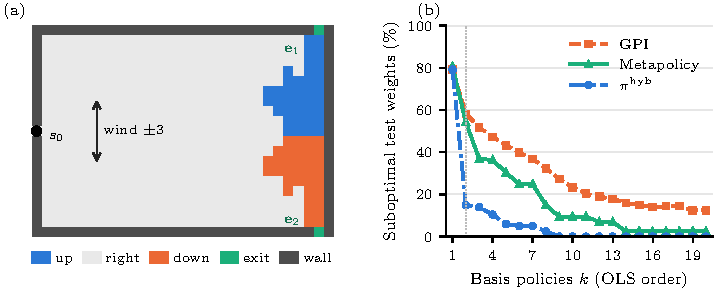
\includegraphics[width=\textwidth]{double_slit.pdf}
    \caption{Double slit domain. (a) Action of the optimal policy for $\mathbf{w} = (0.5, 0.5)$ at each cell: it keeps both exits open and only commits to one of them at the end, which neither corner policy does. (b) Percentage of the 200 held-out weights where GPI, the metapolicy and $\pi^{\mathrm{hyb}}$ are suboptimal, with a basis made of the first $k$ policies found by OLS (exact values). The dotted line marks the two corner policies ($k = 2$).}
    \label{fig:double_slit}
\end{figure}

On the other hand, the extreme policies are not always enough to compose the optimal policy of every task. For example, consider the double slit domain~\cite{kuric_planning_2024} (Figure~\ref{fig:double_slit}a). The agent starts at the left of a corridor, always drifts to the right, and a random wind pushes it up or down until it reaches one of the two exits, $\vphi = \mathbf{e}_1$ at the top and $\vphi = \mathbf{e}_2$ at the bottom. We use a strong wind ($\pm 3$ cells per step) and $\gamma = 0.9$. When both exits have a similar weight, the optimal policy keeps both exits open until late, moving forward and letting the wind decide which exit to take. None of the two corner policies has this behaviour, so the optimal value is up to $20.7\%$ higher than the one of the best corner policy, and the CCS has 181 policies.

We compare three ways of acting with the same basis: GPI (Eq.~\eqref{eq:gpi}), the metapolicy (Eq.~\eqref{eq:metapolicy}) and $\pi^{\mathrm{hyb}}$ (Eq.~\eqref{eq:hyb}) on $200$ random held-out weights $\mathbf{w} = (w_1, 1 - w_1)$. We evaluate each policy exactly and count the weights where it is suboptimal (Figure~\ref{fig:double_slit}b). With only the 2 corner policies, GPI is suboptimal on $58\%$ of the weights and the metapolicy on $54\%$, whereas $\pi^{\mathrm{hyb}}$ is suboptimal on $15\%$, and always by less than $0.02\%$ of the optimal value. The performance of $\pi^{\mathrm{hyb}}$ originates from the possibility of locally taking suboptimal actions while using the metapolicy for future rewards. By contrast, the metapolicy can only switch between the two corner policies at each state. Lastly, GPI evaluates every action following a single base policy afterwards, hence, cannot adapt to a policy that keeps both exits open, see Fig~\ref{fig:double_slit}a. As we add policies in the order OLS finds them, the metapolicy performance greatly surpasses the GPI one. Furthermore, $\pi^{\mathrm{hyb}}$ becomes optimal on all the held-out weights with 9 policies, while with 20 policies the metapolicy is suboptimal on $2.5\%$ of the weights and GPI on $12.4\%$. Notice that the number of suboptimal weights can also increase in GPI, for example, from $k=16$ to $k=17$ it goes $13.9\%$ to $14.4\%$. In general, $\pi^{hyb}$ can replace a large part of the CCS in exchange of performing extra computations for the particular task. In this domain, 9 policies are enough to be optimal on every held-out weight, instead of the 181 required by the full CCS.

\section{Conclusion}\label{sec:conclusions}

We have studied how to speed up the construction of the convex coverage set in three environments, both deterministic and stochastic, and presented a new method that computes the CCS faster than the standard SFOLS algorithm, together with a proof of its convergence. Our method combines the optimal actions of the policies in the basis into a metapolicy that switches between them across the state space. Results show that it speeds up the construction of the CCS and finds the optimal policies with fewer samples on three simple domains. Moreover, our method identifies the base policies of an MDP, which, combined with GPI, can be used to solve new tasks without computing the full CCS. Our results apply to both deterministic and stochastic MDPs, and could be extended to continuous MDPs. In the future, we would like to test the algorithm on more challenging domains, where the rewards and the model have to be learned jointly with the successor features, and to study its behaviour when the successor features are learned with function approximation. Such experiments will establish real benchmarks for practical applications.

\appendix


\section{Convergence of the metapolicy recursion}\label{app:convergence}

We prove the convergence of Algorithm~\ref{alg:metapolicy-ql}, as it is implemented, and then show how to make $\widehat\vpsi$ converge to the SFs of a single policy.

\begin{theorem}\label{thm:sync-convergence}
    Assume that every pair $(s,a)$ is updated infinitely often and that the step sizes satisfy the Robbins--Monro conditions \cite{robbins_stochastic_1951}. Then the policy returned by Algorithm~\ref{alg:metapolicy-ql} is optimal in $\mathcal{M}_{\mathcal{B}}$ after a finite number of updates. Moreover, if the best action of $\mathcal{M}_{\mathcal{B}}$ is unique at every state, then $\widehat\vpsi_t(s,a)$ converges to $\vpsi^{\pi_{\mathrm{meta}}}(s,a)$ for every $(s,a)$.
\end{theorem}

\begin{proof}
    Let $Q_t(s,a) = \widehat\vpsi_t(s,a) \cdot \mathbf{w}$ be the scalarized table at update $t$, $\hat\jmath_t(s)$ the policy maximizer selected at state $s$, and $J^*(s) = \{ j : Q_{V_{\mathrm{meta}}}(s, \pi_j(s)) = V_{\mathrm{meta}}(s) \}$ the base policies whose action is optimal in $\mathcal{M}_{\mathcal{B}}$ at state $s$. To show that the returned policy is optimal, we need to show that it exists $T$ such that $\hat\jmath_t(s) \in J^*(s)$ for $t \geq T$. 


    The update of $\widehat\vpsi$ is a vector operator that is not a contraction in general, since two different tables may bootstrap from different maximizers $\hat\jmath$. However, since $\hat\jmath_t$ maximizes $Q_t$, taking the dot product of the update with $\mathbf{w}$ gives
    \begin{equation*}
        Q_{t+1}(s,a) = Q_t(s,a) + \alpha_t(s,a) \Big[ \vphi(s,a,s') \cdot \mathbf{w} + \gamma \max_j Q_t\big(s', \pi_j(s')\big) - Q_t(s,a) \Big],
    \end{equation*}
    which is Q-learning on $\mathcal{M}_{\mathcal{B}}$ \cite{watkins_q-learning_1992}, extended to the pairs with $a \notin B(s)$, whose entries are updated but never used in the bootstrap. Hence, under the Robbins--Monro conditions and with every pair updated infinitely often, $Q_t \to Q_{V_{\mathrm{meta}}}$ almost surely \cite{tsitsiklis_asynchronous_1994}. 
    
    Now let $\delta = \min_{s} \min_{j \notin J^*(s)} \big( V_{\mathrm{meta}}(s) - Q_{V_{\mathrm{meta}}}(s, \pi_j(s)) \big) > 0$ be the gap between the optimal and the best non-optimal action of $\mathcal{M}_{\mathcal{B}}$. Then there exists $T$ such that $\|Q_t - Q_{V_{\mathrm{meta}}}\|_\infty < \delta/2$ for every $t \geq T$, which implies that for $j \notin J^*(s)$ and $j^* \in J^*(s)$ we then have
    \begin{equation*}
        Q_t(s, \pi_j(s)) < Q_t(s, \pi_{j^*}(s)),
    \end{equation*}
    so the maximizer $\hat\jmath_t(s)$ is in $J^*(s)$, and the greedy policy is optimal in $\mathcal{M}_{\mathcal{B}}$.

    Finally, if the best action is unique at every state, the bootstrap always follows $\pi_{\mathrm{meta}}$ for $t \geq T$, and the update becomes
    \begin{equation*}
        \widehat\vpsi_{t+1}(s,a) = \widehat\vpsi_t(s,a) + \alpha_t(s,a) \big[ \vphi(s,a,s') + \gamma\, \widehat\vpsi_t\big(s', \pi_{\mathrm{meta}}(s')\big) - \widehat\vpsi_t(s,a) \big],
    \end{equation*}
    which is the TD update of the SFs of the fixed policy $\pi_{\mathrm{meta}}$. For the same reasons as $Q_t$, it converges to $\vpsi^{\pi_{\mathrm{meta}}}(s,a)$ almost surely.
\end{proof}

Theorem~\ref{thm:sync-convergence} is enough for the Bellman certificate, which only uses the scalar values $\widehat\vpsi \cdot \mathbf{w}$. However, $\widehat\vpsi$ itself does not necessarily converge. When two actions are tied, their order can change at every update, and if their SFs differ, $\widehat\vpsi$ is pulled towards a different target at each update, while its scalarization still converges. If the SFs of a single metapolicy are needed, for example, to add it to the CCS or to use it with GPI, the ties can be broken easily with a small tolerance and a fixed order over the basis. %We omit the details.

\printbibliography


\end{document}